\documentclass[aspectratio=169, 11pt, xcolor=table]{beamer}

\usepackage{settings/hcmus_beamer}
\input{settings/packages}
% -----------------------------------------------------------------------------
% Description: Custom macros acting as "Decorators" for consistent styling.
% -----------------------------------------------------------------------------

% --- Color Definitions  ---
\definecolor{techBlue}{RGB}{0, 85, 150}
\definecolor{alertRed}{RGB}{200, 30, 30}
\definecolor{codeGreen}{RGB}{0, 150, 80}

% --- Decorator: Text Highlighting ---
% Usage: \highlight{important term}
% Effect: Bold and TechBlue color
\newcommand{\highlight}[1]{\textbf{\textcolor{techBlue}{#1}}}

% --- Math aliases shared with the report ---
\DeclareMathOperator*{\argmax}{arg\,max}
\renewcommand{\vect}[1]{\bm{#1}}
\providecommand{\mat}[1]{\mathbf{#1}}
\providecommand{\scal}[1]{#1}
\providecommand{\trans}{^\top}
\providecommand{\inv}{^{-1}}
\renewcommand{\R}{\mathbb{R}}
\providecommand{\N}{\mathcal{N}}
\providecommand{\given}{\,\middle|\,}

% --- Decorator: Todo Marker ---
% Usage: \todo{Fix this figure}
% Effect: Visible red marker for dev phase
\newcommand{\todo}[1]{\textcolor{alertRed}{\textbf{[TODO: #1]}}}

% --- Component: Paper Title Block ---
% Usage: \paperHeader{Title}{Author}{Conference}
% Description: Standardizes the header for each paper section
\newcommand{\paperHeader}[3]{
    \begin{beamercolorbox}[sep=8pt,center,shadow=true,rounded=true]{title}
        \usebeamerfont{title}#1\par%
        \vskip0.25em%
        {\usebeamerfont{subtitle}\small \textit{#2}}\par%
        {\usebeamerfont{date}\scriptsize \textbf{#3}}
    \end{beamercolorbox}
    \vspace{0.5cm}
}
%-----------------------------------------------------------------------------------------------------
% --- Decorator: Highlighting Key Terms ---
% @param #1: The text to highlight
% Usage: \keyterm{YOLOv11}, \keyterm{GCLI Module}
\newcommand{\keyterm}[1]{\textbf{\textcolor{brown}{#1}}}

% --- Decorator: Paper Citation Header ---
% Description: Creates a standardized header box for introducing a new paper.
% @param #1: Paper Title
% @param #2: Authors
% @param #3: Conference/Year
\newcommand{\paperCard}[3]{
    \begin{beamercolorbox}[sep=0.5em, wd=\textwidth, shadow=true, rounded=true, center]{title}
        \usebeamerfont{frametitle} #1 \par
        \vspace{0.3em}
        \usebeamerfont{subtitle} \scriptsize \textit{#2} \hfill \textbf{#3}
    \end{beamercolorbox}
    \vspace{1em}
}

% --- Decorator: Result Metric Box ---
% Description: A small box to highlight accuracy/F1-score results.
% @param #1: Label (e.g., Accuracy)
% @param #2: Value (e.g., 98.5%)
\newcommand{\resultBox}[2]{
    \begin{beamercolorbox}[colsep*=1ex, rounded=true, shadow=false, center]{block title}
        \small #1 \\
        \LARGE \textbf{#2}
    \end{beamercolorbox}
}
% --- FIX: Define Color locally to avoid "Undefined color" error ---
\definecolor{DeepBlue}{RGB}{0, 51, 102}

\graphicspath{{./images/}{./figures/}{../latex_report/figures/}{../notebooks/artifacts/}}

\titlegraphic{
   
\includegraphics[height=1.5cm]{hcmus_logo}
}
\title[\textbf{GMM with Incomplete Data}]{
    \textbf{Gaussian Mixture Model Clustering\\with Incomplete Data}
}
\subtitle{From paper reproduction to a one-stage view of imputation + clustering}
\author[HCMUS Seminar]{Khang Nguyen \and Nhat Nguyen \and Phuc Nguyen}
\institute[HCMUS]{
    \small Master of Data Science\\University of Science, VNU-HCM
}
\date{\small Seminar slides --- \today}

\setbeamertemplate{navigation symbols}{}
\setbeamertemplate{itemize item}{\color{techBlue}$\blacktriangleright$}
\setbeamertemplate{itemize subitem}{\color{alertRed}$\bullet$}

\setbeamercolor{title}{fg=white,bg=techBlue}
\setbeamercolor{frametitle}{fg=white,bg=techBlue}
\setbeamercolor{block title}{fg=white,bg=techBlue}
\setbeamercolor{block body}{bg=blue!4,fg=black}
\setbeamercolor{alerted text}{fg=alertRed}
\setbeamercolor{palette primary}{bg=techBlue,fg=white}
\setbeamercolor{palette secondary}{bg=black!75,fg=white}
\setbeamercolor{palette tertiary}{bg=black!90,fg=white}

\setbeamertemplate{footline}{
    \hbox{
        \begin{beamercolorbox}[wd=.76\paperwidth,ht=2.6ex,dp=1.1ex,leftskip=0.6cm]{palette primary}
            \small \insertshorttitle
        \end{beamercolorbox}
        \begin{beamercolorbox}[wd=.24\paperwidth,ht=2.6ex,dp=1.1ex,rightskip=0.5cm plus1fil]{palette secondary}
            \small \insertframenumber{} / \inserttotalframenumber
        \end{beamercolorbox}
    }
}

\begin{document}

\begin{frame}[plain]
    \titlepage
\end{frame}

\begin{frame}{Roadmap}
    \tableofcontents[hideallsubsections]
\end{frame}

\section{Motivation}

\begin{frame}[plain,shrink=6]
    \vspace{0.2cm}
    {\Huge \textbf{Missing values do not just remove numbers.}}\\[0.25cm]
    {\LARGE \textcolor{techBlue}{They bend the cluster geometry.}}

    \vspace{0.35cm}
    \begin{columns}[T,onlytextwidth]
        \begin{column}{0.54\textwidth}
            \begin{tikzpicture}[
    x=0.82cm,
    y=0.82cm,
    dotA/.style={circle, fill=techBlue, inner sep=1.8pt},
    dotB/.style={circle, fill=alertRed, inner sep=1.8pt},
    miss/.style={circle, draw=black, fill=white, line width=0.9pt, inner sep=2.2pt},
    impute/.style={cross out, draw=brown, line width=1.1pt, minimum size=5pt, inner sep=0pt},
    axis/.style={-{Latex[length=2.4mm]}, line width=0.6pt, black!65},
    guide/.style={dashed, line width=0.55pt, black!45},
    drift/.style={-{Latex[length=3mm]}, ultra thick, brown}
]
    \fill[blue!6, rounded corners=6pt] (-0.45,-0.55) rectangle (5.15,4.65);
    \fill[red!6, rounded corners=6pt] (3.95,-0.15) rectangle (9.25,5.05);

    \draw[axis] (-0.25,-0.35) -- (9.55,-0.35)
        node[below left=1pt, font=\scriptsize, align=right] {observed coordinate\\$x_o$ known};
    \draw[axis] (-0.25,-0.35) -- (-0.25,5.25)
        node[above, font=\scriptsize, align=center] {missing coordinate\\$x_m$ unknown};

    \foreach \x/\y in {0.35/0.55,1.0/1.1,1.55/0.7,2.25/1.55,1.85/2.35,1.1/2.0,2.8/2.25,2.65/3.1,1.55/3.35,0.75/2.75}
        \node[dotA] at (\x,\y) {};

    \foreach \x/\y in {5.75/0.8,6.45/1.35,7.1/0.9,7.85/1.55,8.35/2.25,7.25/2.45,6.1/2.75,8.05/3.2,6.8/3.65,8.45/0.95}
        \node[dotB] at (\x,\y) {};

    \foreach \x/\y/\yy in {3.45/1.85/2.65,4.75/2.45/3.05,4.25/0.95/1.55} {
        \draw[guide] (\x,-0.18) -- (\x,\yy);
        \node[miss] at (\x,\y) {};
        \node[impute] at (\x,\yy) {};
        \draw[drift] (\x+0.18,\y+0.1) .. controls (\x+0.7,\y+0.7) and (\x+1.1,\yy+0.25) .. (\x+1.65,\yy);
    }

    \node[align=center, font=\bfseries] at (2.0,4.15) {cluster A};
    \node[align=center, font=\bfseries] at (7.1,4.55) {cluster B};

    \node[align=left, font=\scriptsize, anchor=west] at (0.25,5.05)
        {\tikz{\node[miss] {};}\ observed part fixed};
    \node[align=left, font=\scriptsize, anchor=west] at (0.25,4.76)
        {\tikz{\node[impute] {};}\ filled missing part};
    \node[align=center, text=brown, font=\bfseries\scriptsize] at (5.7,0.15)
        {wrong fill changes geometry};
\end{tikzpicture}

        \end{column}
        \begin{column}{0.42\textwidth}
            \vspace{0.1cm}
            \begin{beamercolorbox}[sep=0.8em, rounded=true, shadow=true]{block body}
                \large
                \textbf{If we impute first}\\
                \normalsize the filled values may look plausible\\
                \textbf{but destroy separation.}
            \end{beamercolorbox}

            \vspace{0.2cm}
            \begin{beamercolorbox}[sep=0.8em, rounded=true, shadow=true]{block title}
                \large
                \textbf{Goal}\\
                \normalsize fill the blanks in a way that helps clustering.
            \end{beamercolorbox}
        \end{column}
    \end{columns}
\end{frame}


\begin{frame}[shrink=4]{The Paper in One Sentence}
    \begin{center}
        \begin{beamercolorbox}[sep=0.95em, rounded=true, shadow=true, wd=0.92\textwidth, center]{title}
            \large
            \textbf{Do not separate imputation and clustering.}\\[0.4em]
            \normalsize
            Optimize them \textcolor{alertRed}{together} inside one Gaussian mixture model.
        \end{beamercolorbox}
    \end{center}

    \vspace{0.2cm}
    \begin{tikzpicture}[
    scale=0.88,
    transform shape,
    node distance=0.35cm and 0.45cm,
    box/.style={rounded corners=8pt, draw=black!70, line width=0.9pt, minimum height=1.0cm, align=center, font=\small, inner sep=6pt},
    arrow/.style={-{Latex[length=3mm]}, line width=1.2pt}
]
    \node[font=\Large\bfseries] at (2.5,3.3) {Two-stage};
    \node[box, fill=gray!10, minimum width=2.8cm] (a1) at (1.2,2.2) {Incomplete\\data};
    \node[box, fill=orange!18, minimum width=2.8cm, right=1.0cm of a1] (a2) {Static\\imputation};
    \node[box, fill=gray!10, minimum width=2.8cm, right=1.0cm of a2] (a3) {GMM\\clustering};
    \draw[arrow] (a1) -- (a2);
    \draw[arrow] (a2) -- (a3);
    \node[align=center, text=alertRed, font=\bfseries\small] at (4.35,1.0) {imputation never sees\\the clustering objective};

    \node[font=\Large\bfseries] at (11.0,3.3) {One-stage};
    \node[box, fill=gray!10, minimum width=2.8cm] (b1) at (9.4,2.2) {Incomplete\\data};
    \node[box, fill=blue!12, minimum width=3.5cm, right=1.15cm of b1] (b2) {GMM parameters\\$\alpha_k,\mu_k,\Sigma_k$};
    \node[box, fill=red!10, minimum width=3.4cm, below=0.95cm of b2] (b3) {Missing entries\\$x_{j,m}$};
    \draw[arrow] (b1) -- (b2);
    \draw[arrow] (b2) -- (b3);
    \draw[arrow] (b3.west) .. controls +(180:1.3cm) and +(0:1.3cm) .. (b2.south);
    \node[align=center, text=techBlue, font=\bfseries\small] at (11.2,0.7) {imputation and clustering\\improve each other};
\end{tikzpicture}

\end{frame}

\section{Formulation}

\begin{frame}[shrink=3]{Joint Optimization View}
    \begin{columns}[T,onlytextwidth]
        \begin{column}{0.58\textwidth}
            \[
                \max_{X,\{\alpha_k,\mu_k,\Sigma_k\}_{k=1}^{K}}
                \sum_{j=1}^{n}
                \log\Bigg(
                \sum_{k=1}^{K}\alpha_k \,
                \mathcal{N}(x_j \mid \mu_k, \Sigma_k)
                \Bigg)
            \]

            \[
                \text{s.t. } x_{j,o}=x_{j,o}^{\mathrm{obs}},\qquad
                x_j=\begin{bmatrix}x_{j,o}\\x_{j,m}\end{bmatrix}
            \]

            \vspace{0.25cm}
            \begin{beamercolorbox}[sep=0.8em, rounded=true, shadow=true]{block body}
                \large
                \textbf{The optimization variable is the completed matrix \(X\),}\\
                not only the GMM parameters.
            \end{beamercolorbox}
        \end{column}
        \begin{column}{0.38\textwidth}
            \begin{beamercolorbox}[sep=0.9em, rounded=true, shadow=true]{block title}
                \textbf{Two hidden layers}
            \end{beamercolorbox}
            \vspace{0.15cm}
            \begin{itemize}
                \item \(\gamma_{jk}\): cluster uncertainty
                \item \(x_{j,m}\): feature uncertainty
            \end{itemize}

            \vspace{0.25cm}
            \begin{beamercolorbox}[sep=0.8em, rounded=true, shadow=true]{alerted text}
                \textbf{Observed entries are locked.}\\
                Only the missing block moves.
            \end{beamercolorbox}
        \end{column}
    \end{columns}
\end{frame}


\begin{frame}[shrink=10]{The Three Equations That Matter}
    \small
    \begin{columns}[T,onlytextwidth]
        \begin{column}{0.32\textwidth}
            \begin{beamercolorbox}[sep=0.8em, rounded=true, shadow=true]{block title}
                \textbf{E-step}
            \end{beamercolorbox}
            \[
                \gamma_{jk}=
                \frac{\alpha_k\mathcal{N}(x_j\mid \mu_k,\Sigma_k)}
                {\sum_{\ell=1}^{K}\alpha_{\ell}\mathcal{N}(x_j\mid \mu_{\ell},\Sigma_{\ell})}
            \]
            \vspace{0.1cm}
            \centering
            \small soft cluster membership
        \end{column}
        \begin{column}{0.32\textwidth}
            \begin{beamercolorbox}[sep=0.8em, rounded=true, shadow=true]{block title}
                \textbf{M-step params}
            \end{beamercolorbox}
            \[
                N_k=\sum_{j=1}^{n}\gamma_{jk},\qquad
                \alpha_k=\frac{N_k}{n}
            \]
            \[
                \mu_k=\frac{1}{N_k}\sum_{j=1}^{n}\gamma_{jk}x_j
            \]
            \[
                \Sigma_k=\frac{1}{N_k}\sum_{j=1}^{n}\gamma_{jk}(x_j-\mu_k)(x_j-\mu_k)^\top
            \]
        \end{column}
        \begin{column}{0.32\textwidth}
            \begin{beamercolorbox}[sep=0.8em, rounded=true, shadow=true]{block title}
                \textbf{M-step data}
            \end{beamercolorbox}
            \[
            \begin{aligned}
                x_{j,m}^{\star}
                &=
                \left(\sum_{k=1}^{K}P_{jk}\Lambda_{k,mm}\right)^{-1} \\
                &\quad \cdot
                \sum_{k=1}^{K}
                P_{jk}
                \Big(
                \Lambda_{k,mo}\mu_{k,o}
                +\Lambda_{k,mm}\mu_{k,m}
                -\Lambda_{k,mo}x_{j,o}
                \Big)
            \end{aligned}
            \]
            \centering
            \small precision-weighted conditional reconstruction
        \end{column}
    \end{columns}
\end{frame}

\section{Algorithm}

\begin{frame}[shrink=5]{Alternating Optimization Loop}
    \begin{columns}[T,onlytextwidth]
        \begin{column}{0.58\textwidth}
            \begin{tikzpicture}[
    scale=0.92,
    transform shape,
    node distance=1.2cm,
    stage/.style={rounded corners=10pt, draw=black!75, line width=1pt, minimum width=3.6cm, minimum height=1.2cm, align=center, font=\small\bfseries, inner sep=6pt},
    arrow/.style={-{Latex[length=3mm]}, line width=1.3pt}
]
    \node[stage, fill=orange!20] (init) at (0,0) {1. mean-fill init\\+ KMeans centers};
    \node[stage, fill=blue!14] (estep) at (4.8,0) {2. E-step\\compute $\scal{\gamma}_{jk}$};
    \node[stage, fill=green!16] (mparam) at (4.8,-2.35) {3. parameter M-step\\update $\scal{\alpha}_k,\vect{\mu}_k,\mat{\Sigma}_k$};
    \node[stage, fill=red!12] (mdata) at (0,-2.35) {4. data M-step\\update missing block $\vect{x}_{j,m}$};

    \draw[arrow] (init) -- (estep);
    \draw[arrow] (estep) -- (mparam);
    \draw[arrow] (mparam) -- (mdata);
    \draw[arrow] (mdata) -- (init);

    \node[rounded corners=8pt, draw=black!70, dashed, line width=0.9pt, fit=(estep)(mparam)(mdata), inner sep=12pt] {};
    \node[font=\bfseries] at (2.4,-3.55) {repeat until log-likelihood gain $< \tau$};
\end{tikzpicture}

        \end{column}
        \begin{column}{0.38\textwidth}
            \small
            \begin{beamercolorbox}[sep=0.7em, rounded=true, shadow=true]{block body}
                \textbf{Why it works}
                \begin{itemize}
                    \item every block update pushes the objective upward
                    \item EM handles soft assignments
                    \item closed-form \(x_{j,m}\) update refreshes the surrogate data matrix
                \end{itemize}
            \end{beamercolorbox}

            \vspace{0.25cm}
            \begin{beamercolorbox}[sep=0.65em, rounded=true, shadow=true]{alerted text}
                \textbf{Guarantee:} monotone improvement\\
                \textbf{Reality:} local optimum
            \end{beamercolorbox}
        \end{column}
    \end{columns}
\end{frame}


\begin{frame}[shrink=5]{Why the Missing-Data Update Is the Real Star}
    \begin{center}
        {\large
        Each Gaussian component proposes a local completion.}\\[0.2cm]
        {\large
        Responsibilities decide how much each proposal matters.}
    \end{center}

    \vspace{0.35cm}
    \begin{tikzpicture}[
    scale=0.92,
    transform shape,
    node distance=0.45cm and 0.65cm,
    comp/.style={rounded corners=8pt, draw=black!70, line width=0.9pt, minimum width=3.2cm, minimum height=1.0cm, align=center, font=\small, inner sep=6pt},
    arrow/.style={-{Latex[length=3mm]}, line width=1.1pt}
]
    \node[comp, fill=blue!12] (c1) at (1.8,2.5) {component 1\\$\mu_1,\Lambda_1,\gamma_{j1}$};
    \node[comp, fill=green!13] (c2) at (1.8,1.0) {component 2\\$\mu_2,\Lambda_2,\gamma_{j2}$};
    \node[comp, fill=orange!18] (c3) at (1.8,-0.5) {component $K$\\$\mu_K,\Lambda_K,\gamma_{jK}$};

    \node[comp, fill=gray!10, minimum width=3.4cm, minimum height=3.6cm] (mix) at (7.0,1.0) {solve one linear system\\[0.2em]
    $\displaystyle
    \left(\sum_k P_{jk}\Lambda_{k,mm}\right)x_{j,m}
    =
    \sum_k P_{jk}b_{jk}
    $};

    \node[comp, fill=red!10, minimum width=2.8cm] (out) at (12.15,1.0) {new missing block\\$\bm{x}_{j,m}^{\star}$};

    \draw[arrow] (c1) -- (mix);
    \draw[arrow] (c2) -- (mix);
    \draw[arrow] (c3) -- (mix);
    \draw[arrow, ultra thick] (mix.east) -- (out.west);

    \node[align=center, font=\bfseries, text=techBlue] at (7.0,3.2) {responsibility-weighted fusion};
    \node[align=center, font=\bfseries, text=alertRed] at (12.1,2.5) {cluster-consistent completion};
\end{tikzpicture}


    \vspace{0.15cm}
    \begin{center}
        \large
        \textcolor{alertRed}{Not a generic imputer.}
        It is a \textbf{cluster-aware geometric reconstruction}.
    \end{center}
\end{frame}

\section{Implementation}

\begin{frame}[shrink=7]{How the Repository Mirrors the Math}
    \begin{columns}[T,onlytextwidth]
        \begin{column}{0.56\textwidth}
            \begin{tikzpicture}[
    scale=0.88,
    transform shape,
    node distance=0.55cm and 0.8cm,
    file/.style={rounded corners=8pt, draw=black!75, line width=0.9pt, minimum width=3.8cm, minimum height=0.95cm, align=left, font=\scriptsize, inner sep=6pt},
    arrow/.style={-{Latex[length=3mm]}, line width=1.15pt}
]
    \node[file, fill=blue!10] (core) at (0,0) {\texttt{src/gmm\_missing.py}\\alternating estimator};
    \node[file, fill=green!12, below=of core] (exp1) {\texttt{notebooks/step\_by\_step\_experiment.ipynb}\\single-cycle explanation};
    \node[file, fill=orange!17, below=of exp1] (exp2) {\texttt{notebooks/GMM\_Nhat.ipynb}\\CC GENERAL reproduction};
    \node[file, fill=red!10, below=of exp2] (exp3) {\texttt{src/airplane\_crashes\_pipeline.py}\\real-data workflow};
    \node[file, fill=gray!10, right=1.6cm of exp2, minimum width=3.4cm, minimum height=4.8cm, align=center] (report) {report \& slides\\[0.2em]
    formulas\\figures\\artifacts\\discussion};

    \draw[arrow] (core) -- (report);
    \draw[arrow] (exp1.east) -- (report.west);
    \draw[arrow] (exp2.east) -- (report.west);
    \draw[arrow] (exp3.east) -- (report.west);
\end{tikzpicture}

        \end{column}
        \begin{column}{0.4\textwidth}
            \begin{beamercolorbox}[sep=0.8em, rounded=true, shadow=true]{block title}
                \textbf{Core file}
            \end{beamercolorbox}
            \vspace{0.15cm}
            \texttt{src/gmm\_missing.py}

            \vspace{0.25cm}
            \small
            \begin{beamercolorbox}[sep=0.65em, rounded=true, shadow=true]{block body}
                \textbf{Numerical safeguards}
                \begin{itemize}
                    \item mean fill only for initialization
                    \item KMeans initialization
                    \item covariance ridge regularization
                    \item log-sum-exp in E-step
                    \item fallback when precision blocks are singular
                \end{itemize}
            \end{beamercolorbox}
        \end{column}
    \end{columns}
\end{frame}


\begin{frame}[shrink=4]{Code-to-Equation Mapping}
    \scriptsize
    \renewcommand{\arraystretch}{1.45}
    \begin{tabular}{>{\bfseries}p{0.2\textwidth} p{0.33\textwidth} p{0.38\textwidth}}
        Equation block & Meaning & In code \\
        \toprule
        \(\gamma_{jk}\) & posterior responsibilities & \texttt{\_e\_step()} with log-domain Gaussian scores \\
        \(\alpha_k,\mu_k,\Sigma_k\) & standard GMM M-step & \texttt{\_m\_step\_params()} \\
        \(x_{j,m}^{\star}\) & precision-weighted update for missing entries & \texttt{\_m\_step\_data()} \\
        fit loop & alternating ascent until tolerance & \texttt{fit()} / \texttt{fit\_scale()} \\
        \bottomrule
    \end{tabular}

    \vspace{0.45cm}
    \begin{beamercolorbox}[sep=0.8em, rounded=true, shadow=true]{title}
        \large
        The implementation is not a black box.\\
        \textbf{The paper equations are visible almost line by line.}
    \end{beamercolorbox}
\end{frame}

\section{Results}

\begin{frame}[shrink=5]{Local Reproduction: CC GENERAL}
    \begin{columns}[T,onlytextwidth]
        \begin{column}{0.4\textwidth}
            \small
            \begin{beamercolorbox}[sep=0.7em, rounded=true, shadow=true]{block title}
                \textbf{Setup}
            \end{beamercolorbox}
            \vspace{0.1cm}
            \begin{itemize}
                \item 8,950 customers
                \item 17 numeric features
                \item injected missingness \(\approx 30\%\)
                \item KMeans init + alternating GMM updates
            \end{itemize}

            \vspace{0.2cm}
            \begin{beamercolorbox}[sep=0.6em, rounded=true, shadow=true]{block body}
                \textbf{Observed run}\\
                convergence after \textbf{199} iterations\\
                silhouette score \textbf{0.1489}
            \end{beamercolorbox}
        \end{column}
        \begin{column}{0.56\textwidth}
            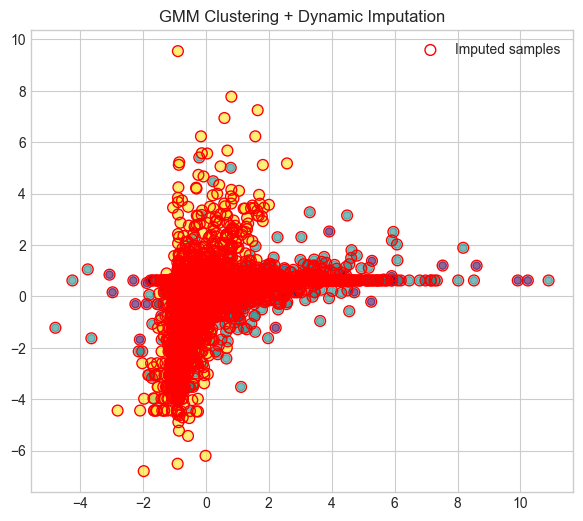
\includegraphics[width=\textwidth]{../latex_report/figures/notebook_exports/GMM_Nhat_cell8_out1.png}
        \end{column}
    \end{columns}
\end{frame}


\begin{frame}[shrink=3]{Application Case: Airplane Crashes}
    \begin{columns}[T,onlytextwidth]
        \begin{column}{0.34\textwidth}
            \begin{beamercolorbox}[sep=0.8em, rounded=true, shadow=true]{block title}
                \textbf{Pipeline}
            \end{beamercolorbox}
            \begin{itemize}
                \item 5,236 usable rows
                \item 6 numeric features
                \item MCAR masking at \(20\%\)
                \item \(\scal{K}=4\) Gaussian components
            \end{itemize}

            \vspace{0.2cm}
            \begin{beamercolorbox}[sep=0.7em, rounded=true, shadow=true]{alerted text}
                RMSE on masked entries\\
                {\LARGE \textbf{20.0588}}
            \end{beamercolorbox}
        \end{column}
        \begin{column}{0.62\textwidth}
            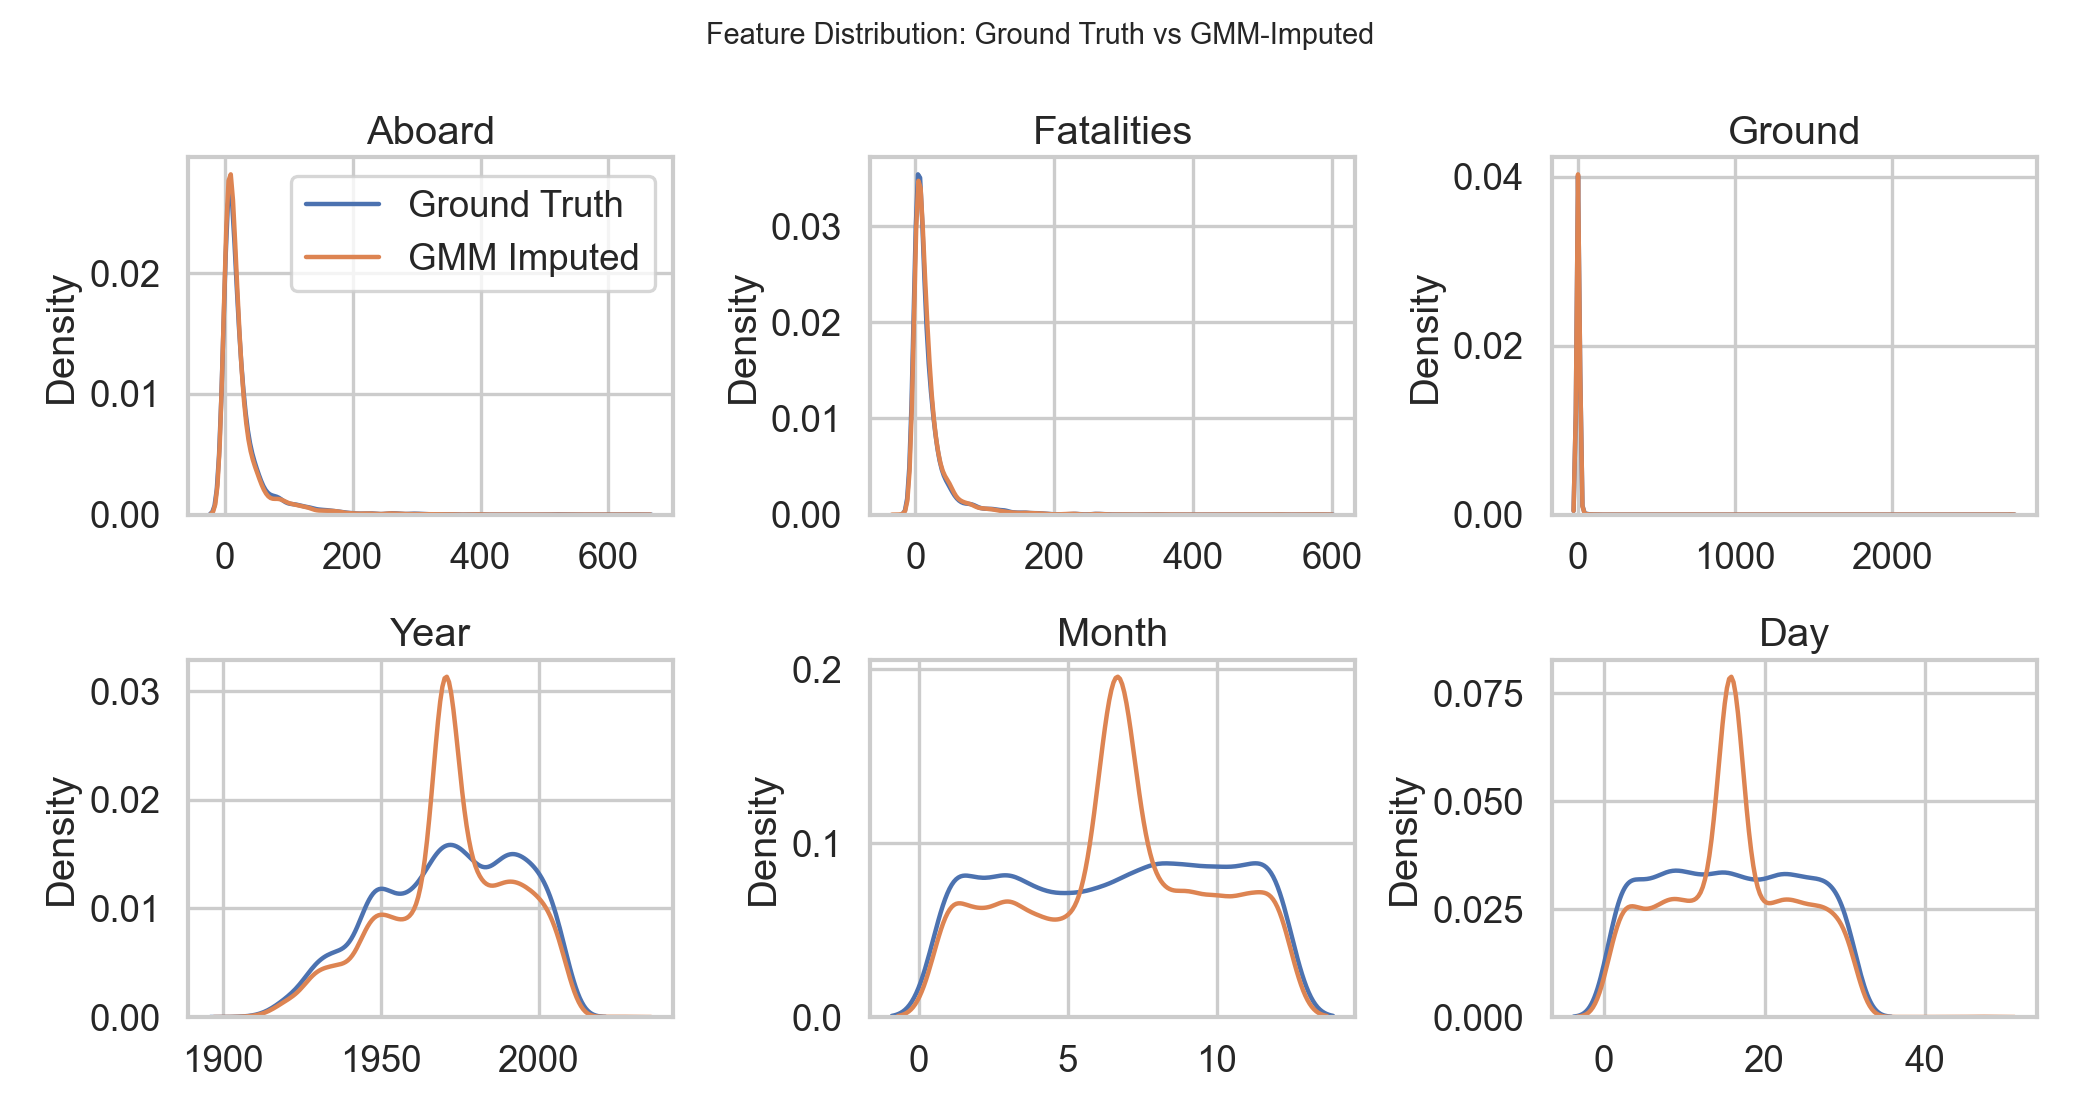
\includegraphics[width=\textwidth]{../latex_report/figures/applications/distribution_comparison.png}
        \end{column}
    \end{columns}
\end{frame}


\begin{frame}[shrink=10]{What the Visual Artifacts Say}
    \begin{columns}[T,onlytextwidth]
        \begin{column}{0.48\textwidth}
            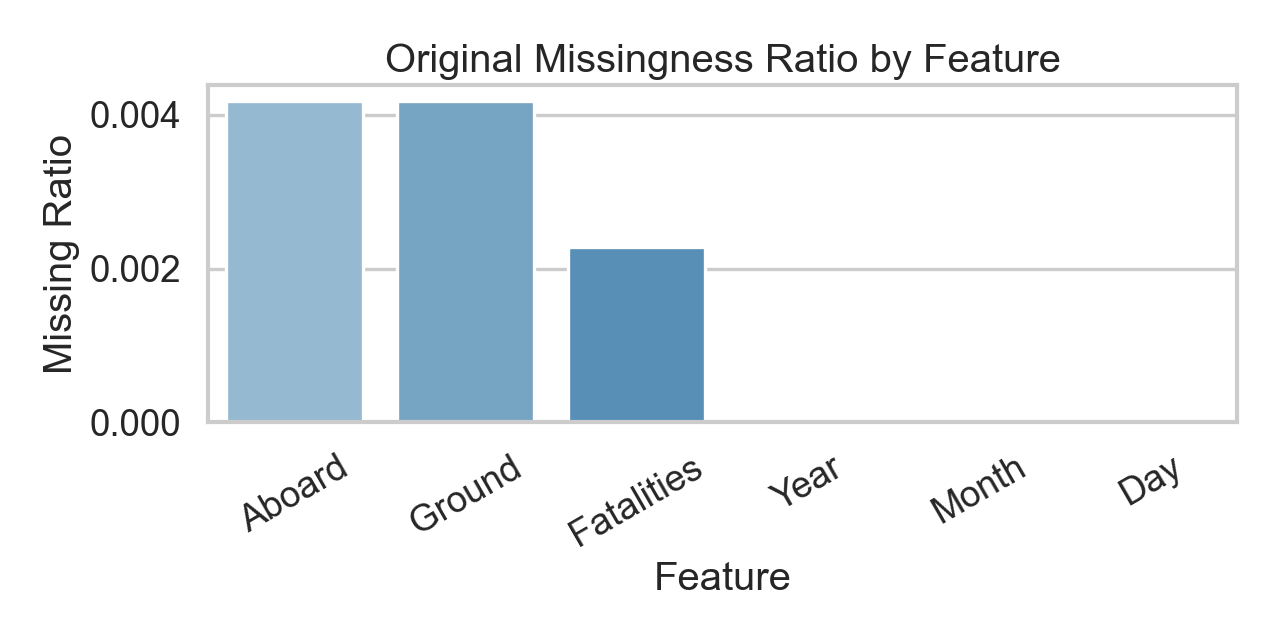
\includegraphics[width=\textwidth]{../latex_report/figures/applications/missingness_ratio.png}
            \vspace{0.1cm}
            \begin{center}
                \small feature-level missingness profile
            \end{center}
        \end{column}
        \begin{column}{0.48\textwidth}
            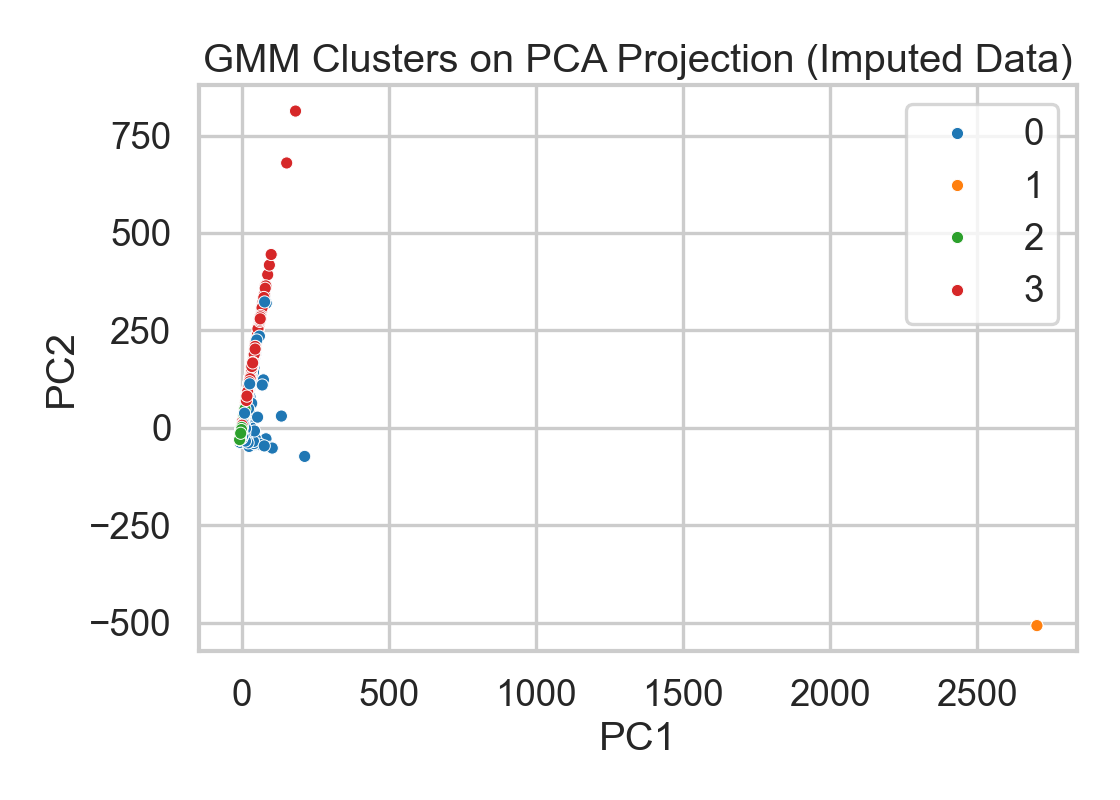
\includegraphics[width=\textwidth]{../latex_report/figures/applications/pca_clusters.png}
            \vspace{0.1cm}
            \begin{center}
                \small geometry after dynamic imputation
            \end{center}
        \end{column}
    \end{columns}

    \vspace{0.25cm}
    \begin{center}
        \large
        \textbf{The method is not only mathematically elegant.}\\
        It survives contact with real, dirty tabular data.
    \end{center}
\end{frame}

\section{Takeaways}

\begin{frame}[shrink=4]{Strengths, Limits, and Research Headroom}
    \begin{columns}[T,onlytextwidth]
        \begin{column}{0.31\textwidth}
            \begin{beamercolorbox}[sep=0.8em, rounded=true, shadow=true]{block title}
                \textbf{Strengths}
            \end{beamercolorbox}
            \begin{itemize}
                \item one-stage objective
                \item cluster-aware imputation
                \item full covariance geometry
                \item monotone ascent behavior
            \end{itemize}
        \end{column}
        \begin{column}{0.31\textwidth}
            \begin{beamercolorbox}[sep=0.8em, rounded=true, shadow=true]{alerted text}
                \textbf{Limits}
            \end{beamercolorbox}
            \begin{itemize}
                \item local optimum only
                \item cubic cost in dimension
                \item sensitive to \(K\), init, regularization
                \item assumes synthetic missingness is informative enough
            \end{itemize}
        \end{column}
        \begin{column}{0.31\textwidth}
            \begin{beamercolorbox}[sep=0.8em, rounded=true, shadow=true]{block body}
                \textbf{Next}
            \end{beamercolorbox}
            \begin{itemize}
                \item diagonal / tied / sparse covariance
                \item automatic model selection
                \item MAR/MNAR-aware extensions
                \item uncertainty-preserving imputation
            \end{itemize}
        \end{column}
    \end{columns}
\end{frame}


\begin{frame}[plain]
    \begin{center}
        \vspace{0.8cm}
        {\Huge \textbf{Take-home message}}\\[0.7cm]

        \begin{beamercolorbox}[sep=1.2em, rounded=true, shadow=true, wd=0.88\textwidth, center]{title}
            \LARGE
            \textbf{For incomplete-data clustering,}\\[0.2cm]
            \textcolor{alertRed}{the best imputation is the one optimized for the clustering objective.}
        \end{beamercolorbox}

        \vspace{1.0cm}
        {\Large Gaussian geometry + alternating optimization + precision-based reconstruction}

        \vfill
        {\Huge \textbf{Q \& A}}
    \end{center}
\end{frame}


\end{document}
